\documentclass[12pt,a4paper]{article}
\usepackage
[
        a4paper,
        left=3cm,
        right=3cm,
        top=4cm,
        bottom=4cm
] {geometry}
\usepackage{wrapfig}
\usepackage{multirow}
\usepackage[utf8x]{inputenc}
\usepackage[romanian]{babel}
\usepackage{lmodern}
\usepackage[pdftex]{graphicx}
\usepackage{caption}
\usepackage{subcaption}
\usepackage[super,comma]{natbib}
\usepackage{indentfirst}
\usepackage{pdfpages}


\usepackage{listings,xcolor}

\definecolor{dkgreen}{rgb}{0,.3,0}
\definecolor{dkblue}{rgb}{0,0,.3}
\definecolor{dkyellow}{cmyk}{0,0,.8,.75}
\definecolor{dkred}{rgb}{.3,0,0}


\lstset{
  language        = php,
  basicstyle      = \scriptsize\ttfamily,
  keywordstyle    = \color{dkblue},
  stringstyle     = \color{dkred},
  identifierstyle = \color{black},
  commentstyle    = \color{dkgreen},
  showspaces	  = false,    
  showstringspaces = false,
  tabsize 		  = 4,
  emph            =[1]{php},
  emphstyle       =[1]\color{black},
  emph            =[2]{if,and,or,else,public,function,\$this,class,implements,return,new},
  emphstyle       =[2]\color{dkblue}
}

\usepackage{paralist}
  \let\itemize\compactitem
  \let\enditemize\endcompactitem
  \let\enumerate\compactenum
  \let\endenumerate\endcompactenum
  \let\description\compactdesc
  \let\enddescription\endcompactdesc
  \pltopsep=\medskipamount
  \plitemsep=1pt
  \plparsep=1pt
\newcommand{\HRule}{\rule{\linewidth}{0.5mm}}

\usepackage{fancyhdr}
\pagestyle{fancy}
\fancyhf{}
\lhead{\textbf{chatbox}: serviciu de mesagerie}
\rhead{\textsc{Atestat la Informatică}}
\rfoot{\thepage}
\lfoot{v03}

\renewcommand*\contentsname{Cuprins}

\begin{document}

\begin{titlepage}
\begin{center}

\textsc{\LARGE Colegiul Național \\[0.5cm] „Mihai Viteazul”}\\[1.5cm]

\textsc{\Large Atestat la Informatică}\\[0.5cm]

\HRule \\[0.4cm]
{ \Huge \bfseries chatbox \\[0.4cm] }

\HRule \\[1.5cm]

\noindent
\begin{minipage}[t]{0.4\textwidth}
\begin{flushleft} \large
\emph{Elev:}\\
\textsc{Vîjială\\Tudor-Gabriel}
\end{flushleft}
\end{minipage}
\begin{minipage}[b]{0.4\textwidth}
\begin{flushright} \large
\emph{Profesor îndrumător:} \\
\textsc{Stan\\ Mihaela-Veronica}
\end{flushright}
\end{minipage}

\vfill

% Bottom of the page
{\small 18 mai 2015}

\end{center}
\end{titlepage}

\newpage
\section{Introducere}


\hspace{-26px}
\begin{tabular}{l l l l}
\texttt{chat} & --  \textit{s.f.} & conversație informală &\\
\texttt{to box} & --  \textit{v. tranz.} & a inchide, a separa (într-o cutie)&\\
& & & -- Dicționar englez-român\\ %\hline
\end{tabular}

\vfill
{\large \textbf{Chatbox} este un serviciu de mesagerie Web.}

\begin{figure}[h]
	\centering
	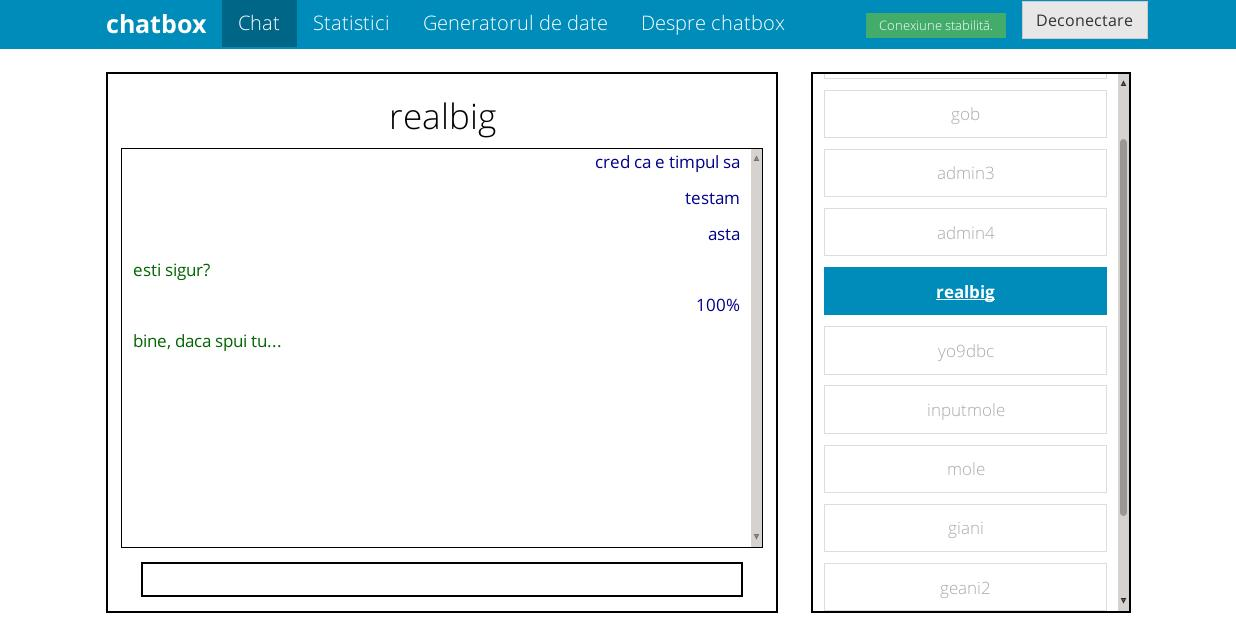
\includegraphics[width=150mm]{img/over.jpg}
	\vspace{-15px}
	\caption{Interfața modulului de mesagerie}
	\vspace{-15px}
	\label{fig:overview}
\end{figure}

\vspace{3mm}
Acest proiect a fost inspirat de serviciile de „mesagerie instantanee”
precum \textit{Y!Messenger}, \textit{Google Talk} sau 
\textit{Facebook Messenger}.
%\vfill

\begin{figure}[h!]
        \centering
        \begin{subfigure}[b]{0.45\textwidth}
                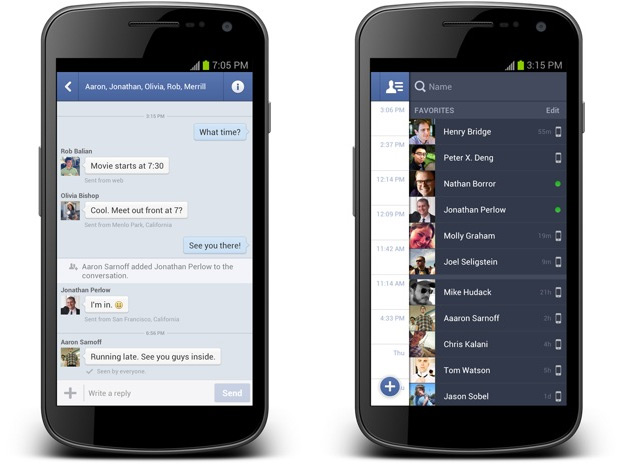
\includegraphics[height=5cm]{img/fb_mess.jpg}
                \caption{Facebook Messenger}
               % \label{fig:gull}
        \end{subfigure}%
        ~ \qquad 
        \begin{subfigure}[b]{0.45\textwidth}
                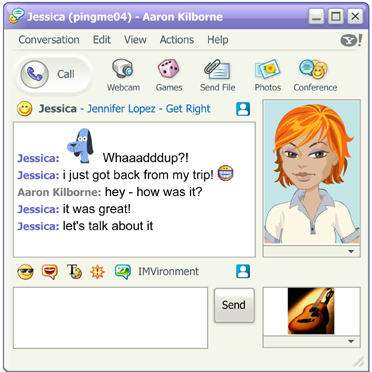
\includegraphics[height=5cm]{img/yahoo_mess.jpg}
                \caption{Yahoo! Messenger}
                %\label{fig:tiger}
        \end{subfigure}
        \caption{Servicii de mesagerie digitală}%\label{fig:animals}
\end{figure}



În prezent, \textbf{Chatbox} poate fi accesat la adresa
\textbf{penultim.ddns.net/chatbox}.



\newpage
\section{Resurse logice}
\textit{Resursele logice} sunt componentele software ale calculatorului care au funcții de administrare a resurselor și a datelor.

În cazul proiectului \textbf{Chatbox}, acestea reprezintă mijlocul prin care
pagina Web este programată, monitorizată și administrată.

\subsection{Sistemul MySQL}
MySQL\cite{mysql} este cel mai folosit SGBD\citep{sgbd} open-source, 
la ora actuală. Produs inițial de compania suedeză MySQL AB 
și distribuit sub Licența Publică Generală GNU\cite{free}, 
in prezent MySQL este dezvoltat
de Corporația Oracle.

Ca instrument de management pentru bazele de date MySQL
este folosită o aplicație PHP numită phpMyAdmin.

\subsection{Limbajul PHP}
Limbajul de programare PHP\citep{php} este folosit pe scară largă 
în dezvoltarea paginilor și aplicațiilor web.

Se folosește în principal înglobat în codul HTML, dar poate fi 
utilizat și pentru programarea aplicațiilor CLI (linie de comandă).

PHP este disponibil sub Licenṭa PHP ṣi Free Software Foundation 
îl consideră a fi un software liber\citep{free}.

\subsubsection{Librăria PDO}
PHP Data Objects\citep{pdo} este o componentă PHP ce permite accesarea unor SGBD din
programe PHP. \textbf{Chatbox} folosește  în mod exclusiv componenta PDO pentru 
accesarea bazei de date. 

\subsubsection{Librăria Ratchet}
Websocket\citep{websocket} este un protocol ce furnizează o conexiune full-duplex prin o legatură TCP. Tehnologia Websocket a fost dezvoltată odată cu inițiativa de 
inovare HTML5. 

Folosind tehnologia Websocket, se pot trimite date în timp real între 
client și server. \textbf{Chatbox} foloseste acest protocol pentru
transmiterea instantanee a mesajelor și a datelor.

Ratchet\citep{ratchet} este o librărie ce permite utilizarea protocolului 
Websocket în limbajul PHP.

\subsection{Limbajul JavaScript}
JavaScript (sau ECMAScript) este un limbaj de programare orientat pe obiecte\citep{javascript} ce rulează  în browserele utilizatorilor. 

Limbajul este binecunoscut pentru folosirea sa în construirea paginilor Web. În ciuda numelui și a unor similarități în sintaxa codului, între \textit{JavaScript} și limbajul \textit{Java} nu există nicio legătură.

\subsubsection{Tehnica AJAX}
O tehnică de construire a paginilor web tot mai întâlnită în ultimul timp este AJAX, abreviere de la „Asynchronous JavaScript and XML”. Această tehnică constă în executarea de cereri HTTP în fundal, fără a reîncărca toată pagina Web, și actualizarea numai a anumitor porțiuni ale paginii.

\textbf{Chatbox} folosește tehnica AJAX pentru a încărca o multitudine de
elemente, precum textul mesajelor primite sau lista de utilizatori activi. 

\subsubsection{Librăria jQuery}
jQuery\citep{jquery} este o platformă de dezvoltare JavaScript, concepută pentru a ușura și îmbunătăți procese precum traversarea arborelui DOM\citep{dom} în HTML, managementul evenimentelor, animații și cereri de tip AJAX.

\subsubsection{Librăria chart.js}
Chart.js\cite{chartjs} este o librărie JavaScript ce permite afișarea 
unor grafice în mod dinamic. Graficele sunt redimensionate, la nevoie, după 
mărimea ecranului clientului. 

Proiectul \textbf{Chatbox} foloseste chart.js pentru afișarea rezultatelor
numerice ale unor interogări SQL și pentru vizualizarea de statistici.

\subsubsection{Librăria Bootstrap}
Bootstrap este cel mai popular framework de HTML, CSS și JavaScript dedicat dezvoltării proiectelor Web. 

Bootstrap permite aranjarea elementelor grafice într-un mod potrivit mărimii ecranului vizitatorului. Astfel, site-ul va fi afișat corect atât pe calculatoare Desktop, cât și pe tablete sau telefoane.

\subsection{Limbajul Python}
Python este un limbaj de programare dinamic multi-paradigmă\cite{python}, creat în 1989 de către programatorul olandez Guido van Rossum\cite{pythonWiki}.

Python pune accent pe acuratețea și simplitatea codului, iar sintaxa sa le permite dezvoltatorilor să exprime idei programatice într-o manieră cât mai clară și mai concisă.

Generatorul de date folosit de \textbf{Chatbox} este implementat în Python 3.

\subsection{Serverul Linux}
Codul proiectului \textbf{Chatbox} rulează pe un calculator personal
 \textit{HP Compaq 6005 Pro}
care servește, printre altele, drept server Web. 
Sistemul are urmatoarele caracteristici:
\begin{itemize}
  \item Procesor: AMD Athlon II X2 2.8GHz
  \item Memorie: 2GB RAM DDR3
  \item Hard Drive: 2TB, Samsung
  \item Placă de rețea: 100Mbps
  \item Sistem de operare: Debian 8
\end{itemize}

Pentru a dispune de o adresă permanentă a acestui server, 
am folosit serviciile de DNS dinamic ale companiei NoIP\cite{noip}.

\subsubsection{Sistemul de operare Debian 8}
Debian\cite{debian} este un sistem de operare compus din software liber\cite{free} și reprezintă totodată o distribuție populară și foarte influentă între distribuțiile GNU/Linux.

Versiunea 8 a sistemului de operare este cunoscută în prezent sub 
numele de \textit{testing}. Pachetele de software pentru versiunea 
\textit{testing} sunt, după cum sugerează și numele, în curs de testare.
Totuși, sunt suficient de stabile pentru modul  în care 
este utilizat acest sistem.

\subsubsection{Serverul HTTP Apache 2}
Apache este un server HTTP open-source. Acesta reprezintă standardul în 
industria de Web Hosting, fiind cel mai folosit server HTTP, susținând 
53.34\% din site-urile Web\cite{apache53}.

\subsubsection{Sistemul de monitorizare daemontools}
Daemontools\cite{daemon} este o colecție de instrumente software folosite pentru 
controlul și monitorizarea serviciilor UNIX. 

Daemontools este folosit de \textbf{Chatbox} pentru a monitoriza serverul 
de \textit{websockets} și a-l reporni  în eventualitatea unei erori.

\subsection{Procesorul \LaTeX}
Acest document a fost compus folosind procesorul ~ \LaTeX ~ care permite pregătirea
acestuia pentru tipărire în format electronic,
cu ajutorul limbajului de programare ~ \TeX.



\newpage
\section{Descrierea proiectului}
\textbf{Chatbox} a fost conceput ca un mijloc de a învăța atât despre programarea
Web în general, cât și despre sistemele de transmitere de date în timp real.

\subsection{Baza de date}
Sistemul \textbf{Chatbox} stochează  în baza de date toate detaliile interacționării
utilizatorilor cu acesta. Informațiile sunt atât de conținut 
(mesajele trimise), cât și metadate (\textit{exemplu}: ce sistem de operare a fost folosit de către un anumit utilizator).

%Schema bazei de date MySQL este compusă din 3 tabele: 
%\texttt{utilizatori}, \texttt{sesiuni} și \texttt{mesaje}.

Structura tabelelor este următoarea:
\begin{figure}[h]
\centering
\texttt{%
	\begin{tabular}{| l | l | l | p{5.5cm} |} \hline
	\textbf{Tabel} & \textbf{Nume} 			& \textbf{Tip}		  		& \textbf{Observații}\\ \hline
	\multirow{6}{*}{utilizatori}
	&id           	& bigint(20) &  PK: identificator numeric\\
	&nume         	& tinytext            & numele utilizatorului\\	
	&hash         	& varchar(512)        & hash-ul parolei\cite{passwordhash}\\
	&data\_ire		& datetime            & data înregistrării\\
	&activ         	& tinyint(1)          & 1 - activ, 0 - inactiv\\ \hline
	\multirow{8}{*}{sesiuni}
	& id\_sesiune    & bigint(20) & PK\\
& cheie\_sesiune & varchar(512)        & \\
& id\_utilizator & bigint(20)          & FK\\
& inceput       & datetime            & momentul de log-in\\
& sfarsit       & datetime            & momentul de log-out\\
& adresa\_ip     & tinytext            & \\
& browser       & tinytext            & browserul folosit\\
& platforma     & tinytext            & SO folosit\\ \hline
\multirow{8}{*}{mesaje}
& id\_mesaj      & bigint(20) & PK \\
& id\_expeditor  & bigint(20)          & FK \\
& id\_destinatar & bigint(20)          & FK \\
& text          & text                & conținutul mesajului \\
& data          & datetime            & momentul expedierii \\
& citit         & tinyint(1)          & 1 - citit, 0 - necitit\\ \hline
	\end{tabular}
}
\vspace{-8px}
\caption{Structura bazei de date}
\vspace{-20px}
\end{figure}

\subsection{Diagrama de secvență}
Unified Modeling Language (prescurtat UML) este un limbaj standard pentru descrierea de modele și specificații pentru software\cite{uml}.

Urmatoarea diagramă descrie interacțiunile dintre cele patru componente 
de bază ale sistemului: browserul utilizatorului, serverul Web, baza de date și 
serverul Websocket.

%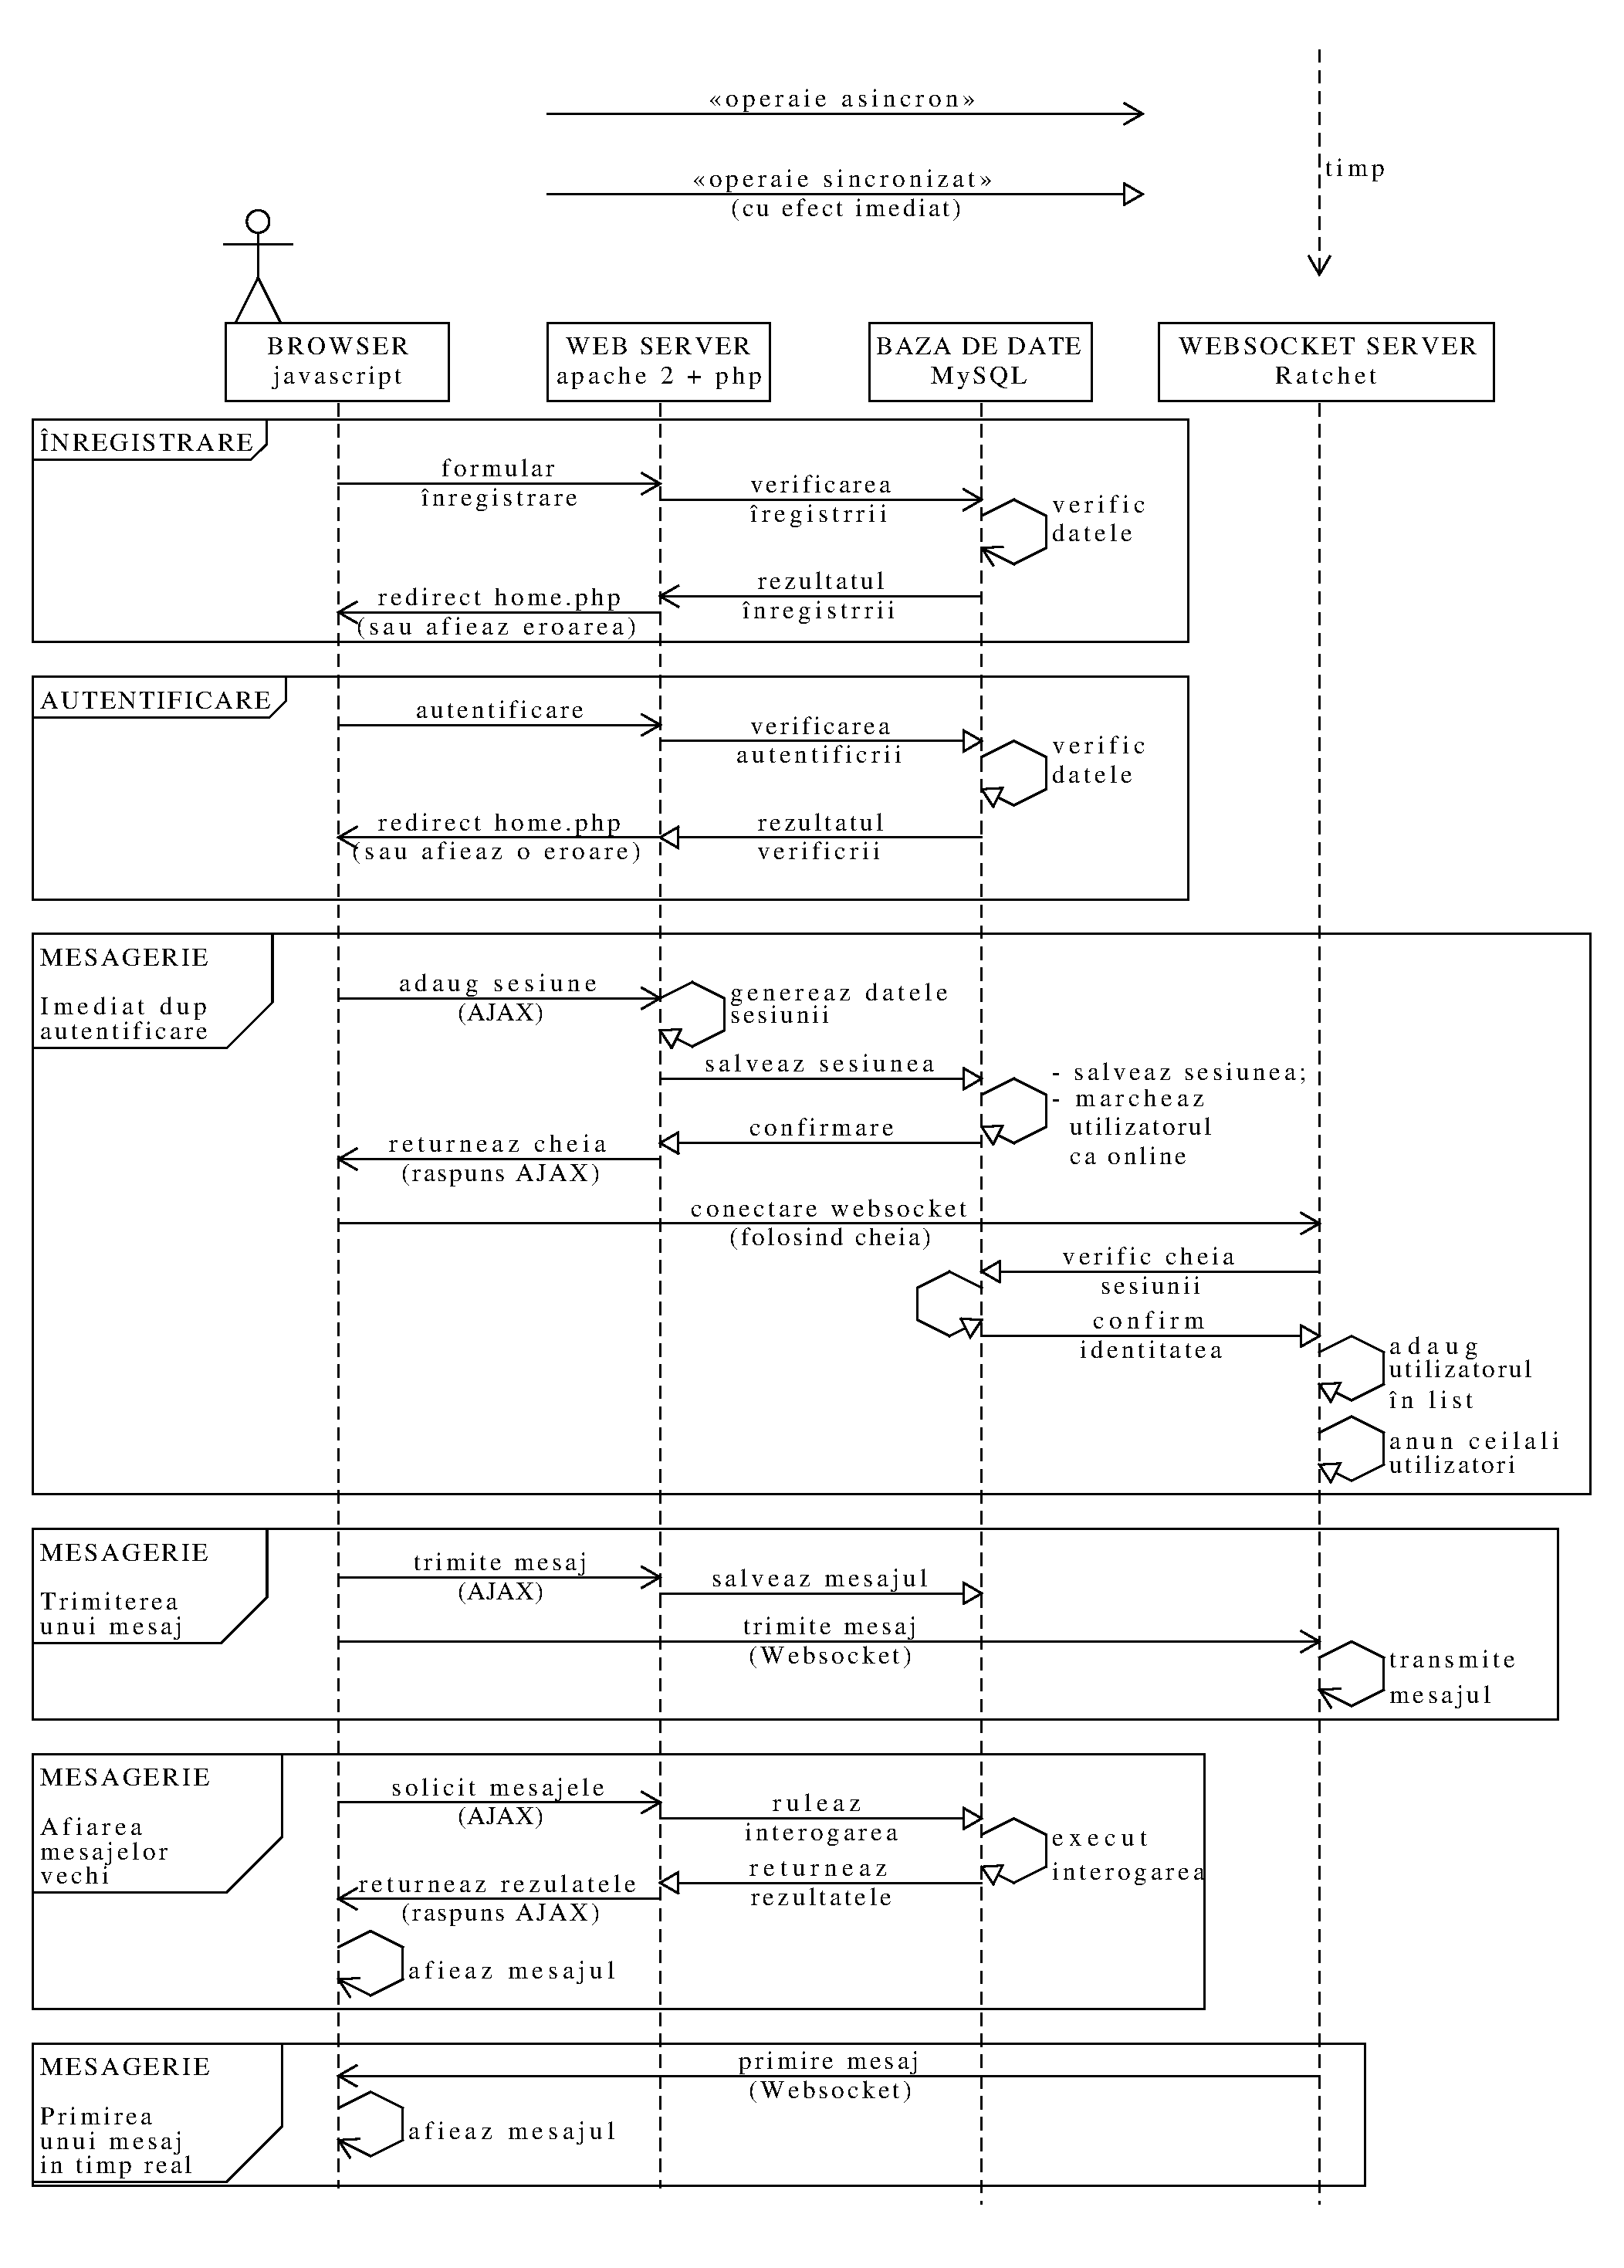
\includepdf[pagecommand={\pagestyle{fancy}},scale=0.75]{diagrame/chat_sequence.pdf}
\newpage
	\begin{figure}[!ht]
	\centering
	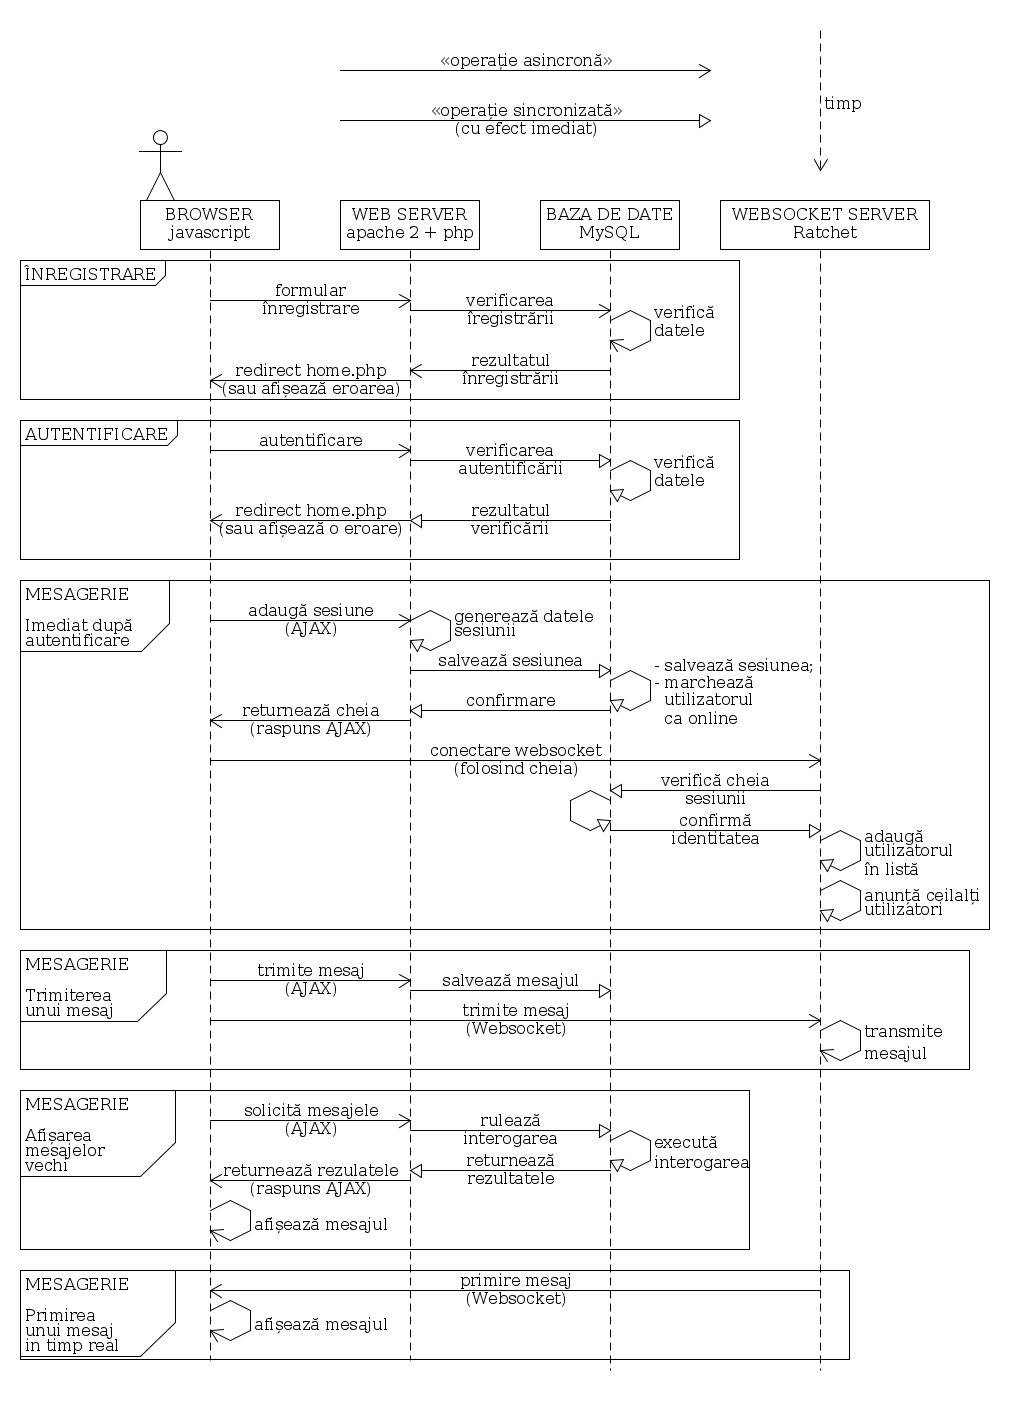
\includegraphics[height=0.97\textheight]{diagrame/chat_sequence.png}
	\vspace{-20pt} 
	\caption{Diagrama de secvență pentru modulul de mesagerie \label{overflow}}
	\vspace{-20pt} 
\end{figure}

\subsection{Sistemul de autentificare}
Pentru a folosi serviciul de mesagerie, un utilizator trebuie să fie înregistrat și autentificat. Înregistrarea este liberă; singurele date necesare sunt numele de utilizator
și o parolă.

\begin{figure}[h!]
        \centering
        \begin{subfigure}[b]{0.45\textwidth}
                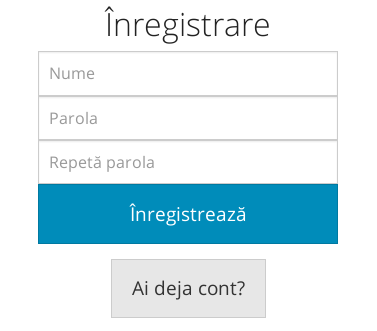
\includegraphics[height=5cm]{img/inreg.png}
                \caption{Interfața de înregistrare}
               % \label{fig:gull}
        \end{subfigure}%
        ~ \qquad 
        \begin{subfigure}[b]{0.45\textwidth}
                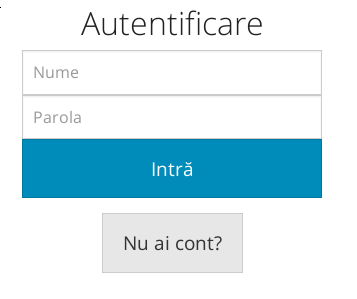
\includegraphics[height=5cm]{img/auth.png}
                \caption{Interfața de autentificare}
                %\label{fig:tiger}
        \end{subfigure}
        \caption{Formulare de înregistrare și autentificare}%\label{fig:animals}
\end{figure}

 

În cazul  în care apar erori în procesul creării contului sau în procesul autentificării,
utilizatorul va primi o înștiințare pe fundal roșu care explică situația.

Aceste verificări se fac pe server,  în câte un script PHP, pentru verificarea autentificării, respectiv a înregistrării. 

\begin{figure}[h!]
        \centering
        \begin{subfigure}[b]{0.35\textwidth}
                
\includegraphics[height=2.5cm]{img/fail1.png}
                \caption{la autentificare}
               % \label{fig:gull}
        \end{subfigure}%
        ~ \qquad 
        \begin{subfigure}[b]{0.55\textwidth}
                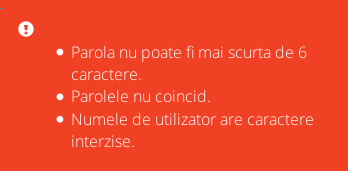
\includegraphics[height=3.2cm]{img/fail2.png}
                \caption{la înregistrare}
                %\label{fig:tiger}
        \end{subfigure}
        \caption{Posibile erori după completarea eronată a formularelor}%\label{fig:animals}
\end{figure}

Paginile accesate pentru autentificare și înregistrare sunt \texttt{autentificare.php} și
\texttt{inregistrare.php}. Verificarea fiecărui procedeu este efectuată în programele
\texttt{php/verifica\_autentificare.php} și \texttt{php/verifica\_inregistrare.php}.

\vfill

Pentru exemplificare este atașată mai jos sursa fișierului responsabil de verificarea autentificării:

\begin{lstlisting}
<?php
/* php/verifica_autentificare.php */
require_once('functii.php');
require_once("bd_functii.php");
session_start();
unset($_SESSION['ERORI']);

$mesaje_erori = array();
$avem_eroare = false;

$nume = $_POST['nume'];
$parola = $_POST['parola'];

if ($nume == '') {
    $avem_eroare = true;
    $mesaje_erori[] = "Numele de utilizator lipseste. ";
}
if ($parola == '') {
    $avem_eroare = true;
    $mesaje_erori[] = "Parola lipseste. ";
}
if (preg_match('/\\W|_/', $nume)) {
    $avem_eroare = true;
    $mesaje_erori[] = "Numele de utilizator contine caractere interzise. ";
}
if ($avem_eroare == true) {
    $_SESSION['ERORI'] = $mesaje_erori;
    redirect("../autentificare.php");
} else {
    unset($_SESSION['ERORI']);
}

conectare_baza_date();
$query = "SELECT * FROM utilizatori WHERE nume=?";
$fetch = interogare_bd($query, $nume);
$hash = $fetch['hash'];

if (password_verify($parola, $hash)) {
    // autentificare ok
    $_SESSION['ID'] = $fetch['id'];
    $_SESSION['NUME'] = $fetch['nume'];
    redirect("../home.php");
} else {
    // autentificare esuata
    $mesaje_erori[] = "Autentificare esuata";
    $_SESSION['ERORI'] = $mesaje_erori;
    redirect("../autentificare.php");
}
\end{lstlisting}

\newpage
\subsection{Interfață grafică și design}
Pentru construirea interfeței grafice și a design-ului am folosit librăria Bootstrap\cite{bootstrap} și adiții din partea site-ului Bootswatch\cite{bootswatch}.

\textbf{Chatbox} abordează un stil minimalist, folosind doar culori elementare: 
albastru pentru interfață și meniu, roșu pentru erori. Culorile sunt alese folosind 
pachetul Yeti\cite{yeti} din colecția Bootswatch.

\subsubsection{Funcția de remodelare}

\begin{wrapfigure}{r}{0.23\textwidth} %this figure will be at the right
    \centering
    \vspace{-20px}
    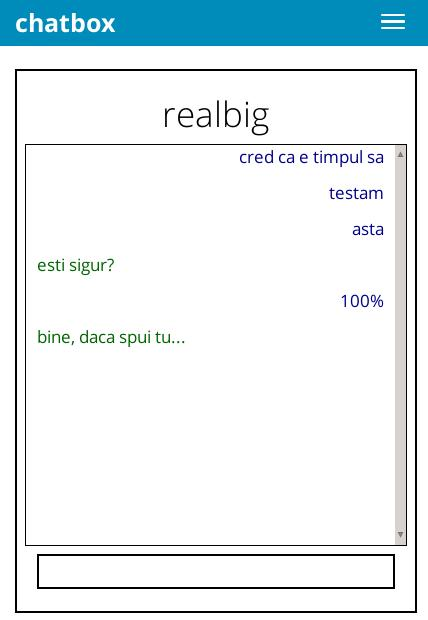
\includegraphics[width=0.23\textwidth]{img/chat_mobil.jpg}
	\caption{Interfața modulului de mesagerie, pe un terminal mobil}
	\label{fig:mobil}
\end{wrapfigure}

Bootstrap are la centrul său conceptul de „responsive web design\cite{rwd}”, adică modelarea componentelor
vizuale pentru a „răspunde” cât mai bine la tipul de terminal folosit. Astfel, site-ul va avea altă structură dacă este afișat pe un Desktop PC, decât dacă este afișat pe un ecran de telefon.

Pentru exemplificare, comparați modul de afișare al modulului de mesagerie, între 
raspunsul site-ului pentru un Desktop PC (pagina \pageref{fig:overview}, Figura \ref{fig:overview}) și un ecran de telefon mobil (Figura \ref{fig:mobil}).

\subsubsection{Bara de navigație}
Bara albastră din partea de sus a ecranului este prezentă în fiecare pagină  
a site-ului \textbf{Chatbox} și se numește \textit{bară de navigație}. Aceasta 
este folosită ca meniu pentru site, aici fiind afișate toate secțiunile de interes
pe care utilizatorii le pot vizita. 

\begin{figure}[!h]
	\centering
	
\includegraphics[width=\textwidth]{img/meniu_mare.jpg}
	\vspace{-15px}
	\caption{Bara de navigație, afișată pe un sistem Destktop PC.}
\end{figure}

\begin{figure}[!h]
	\centering
	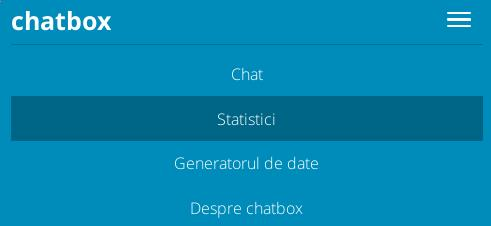
\includegraphics[width=0.45\textwidth]{img/meniu_mobil.jpg}
	%\vspace{-15px}
	\caption{Bara de navigație, afișată pe un terminal mobil.}
	\label{fig:nav-mobil}
\end{figure}

Pentru ecrane de rezoluție mică, precum cele de telefon sau tabletă, bara de navigație își schimbă forma și poate fi extinsă sau micșorată la nevoie, 
folosind butonul din dreapta-sus [Figura \ref{fig:nav-mobil}].

\subsection{Sistemul de mesagerie}
Funcționalitatea centrală a proiectului este sistemul de mesagerie în timp real. 
Acesta permite trimiterea de mesaje text către orice alt utilizator al \textbf{Chatbox}.

\subsubsection{Interfața specifică}
Ca să păstreze stilul minimalist, interfața are un design simplu și funcțional. 
Ecranul este împărțit între o listă cu ceilalți utilizatori și o căsuță unde apar mesajele
din conversația curentă. 

\begin{figure}[h!]
        \centering
        \begin{subfigure}[b]{0.45\textwidth}
                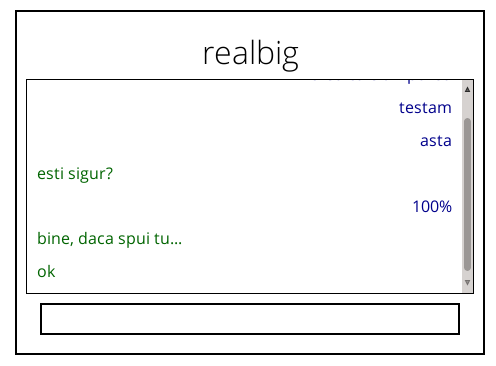
\includegraphics[height=4.5cm]{img/zona.png}
                \caption{Căsuța cu mesaje}
               % \label{fig:gull}
        \end{subfigure}%
        ~ \qquad 
        \begin{subfigure}[b]{0.35\textwidth}
                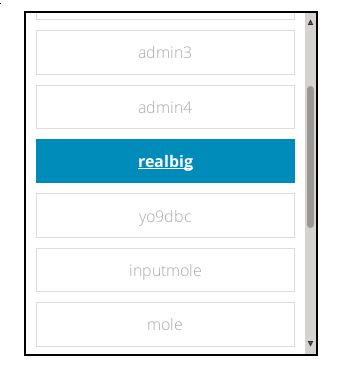
\includegraphics[height=4.5cm]{img/lista.png}
                \caption{Lista de utilizatori}
                %\label{fig:tiger}
        \end{subfigure}
        \vspace{-7px}
        \caption{Interfața sistemului de mesagerie}%\label{fig:animals}
\end{figure}

Se poate selecta un alt utilizator, folosind un simplu \textit{click}. Utilizatorul activ este afișat în partea de sus a căsuței cu mesaje. 

\begin{figure}[h!]
        \centering
        \begin{subfigure}[b]{0.25\textwidth}
                
\includegraphics[height=0.7cm]{img/lista_offline.jpg}
                \caption{Utilizator offline}
               % \label{fig:gull}
        \end{subfigure}%
        ~ \qquad 
        \begin{subfigure}[b]{0.25\textwidth}
                
\includegraphics[height=0.7cm]{img/lista_mesaj.jpg}
                \caption{Mesaj nou}
               % \label{fig:gull}
        \end{subfigure}%
        ~ \qquad 
        \begin{subfigure}[b]{0.25\textwidth}
                
\includegraphics[height=0.7cm]{img/lista_online.jpg}
                \caption{Utilizator online}
                %\label{fig:tiger}
        \end{subfigure}
        \vspace{-7px}
        \caption{Elementele listei de utilizatori}%\label{fig:animals}
\end{figure}


Trimiterea unui mesaj se poate realiza prin tastarea acestuia în zona de trimitere și prin 
apăsarea tastei \textit{enter}. Din acest motiv, am considerat că era inutil să se 
adauge și un buton care împlinește același rol. Alegerea a fost inspirată din design-ul 
chat-ului implementat de Facebook. 

Mesajele se pot trimite doar dacă clientul este conectat la serverul de \textit{websocket}, 
care are rolul de a primi și de a trimite mai departe conținutul mesajelor de la un 
utilizator la altul, în timp real. \textbf{Chatbox} anunță utilizatorii dacă sunt conectați 
printr-un element de afișaj.

\begin{figure}[!h]
	\centering
	\vspace{-7px}
	
\includegraphics[width=0.4\textwidth]{img/chat_butoane.jpg}
	\vspace{-7px}
	\caption{Butoanele specifice interfeței de chat}
\end{figure}

\subsubsection{Serverul de websockets}
După cum a fost explicat mai sus, protocolul este folosit pentru a transmite mesajele 
de la expeditor la destinatar, într-un timp cât mai scurt.  Acest procedeu se realizează, 
evident, doar dacă atât expeditorul cât și destinatarul sunt conectați la server. 

Librăria \textit{Ratchet} este folosită pentru a implementa acest server, 
ce rulează la adresa paginii \textbf{Chatbox}, pe portul \texttt{8091}.

\begin{lstlisting}
<?php
/* php/websocket/ChatListener.php */

class ChatListener implements MessageComponentInterface {
	// Lista cu clienti activi
    protected $clienti;
    protected $legaturi = array(0 => null); 

    public function __construct() {
        $this->clienti = new \SplObjectStorage;
        echo 'ChatListener initializat!\n';
    }

	// Trimite mesajul $mesaj de la expeditor.
    function trimite_mesaj($expeditor, $mesaj) {
        $trimis = false;
        $mesaj['id_expeditor'] = $this->legaturi[$expeditor->resourceId]['id'];
        foreach ($this->clienti as $client) {
            if (/* ... */ ) {
                $client->send(json_encode($mesaj));
                $trimis = true;
            }
        }
        return $trimis;
    }

	// Initializeaza o sesiune folosind cheia primita.
    function initializeaza_sesiune($utilizator, $cheie) {
        $transmisie = array(/* ... */);
        $transmisie_text = json_encode($transmisie);
        foreach ($this->clienti as $client) {
            if ($utilizator !== $client) {
                $client->send($transmisie_text);
            }
        }
        $q = "UPDATE utilizatori SET activ = 1 WHERE id = ?";
        inserare_bd($q, $id);   deconectare_baza_date();
    }

	// Inchide o sesiune si seteaza utilizatorul ca fiind inactiv.
    function sfarseste_sesiune($conexiune, $id, $cheie) {
        $transmisie = array(/* ... */);
        $transmisie_text = json_encode($transmisie);
        foreach ($this->clienti as $client) {
            if ($conexiune !== $client) {
                $client->send($transmisie_text);
            }
        }
        inserare_bd("UPDATE utilizatori SET activ = 0 WHERE id = ?", $id);
        inserare_bd("UPDATE sesiuni SET sfarsit = ? WHERE cheie_sesiune = ?", 
        			 array(\acum(), $cheie));
        deconectare_baza_date();
    }

	// Rulat in momentul in care un utilizator se 
	// conecteaza la server. 
    public function onOpen(ConnectionInterface $conexiune) {
        $this->clienti->attach($conexiune);
    }

	// Rulat in momentul in care un utilizator trimite un mesaj
	// catre server. Acest mesaj poate fi de doua tipuri
	// (trimitere de mesaj text, sau operatiune). 
    public function onMessage(ConnectionInterface $expeditor, $mesaj) {
        $resId = $expeditor->resourceId;
        $date = json_decode($mesaj, true);

        switch ($date['operatie']) {
            case 'trimitere':
                $this->trimite_mesaj($expeditor, $date);
                break;
            case 'initializare':
                $this->initializeaza_sesiune(
                	$expeditor, $date['cheie']);
                break;
        }
    }

	// Rulat in momentul in care un utilizator se 
	// deconecteaza de la server. 
    public function onClose(ConnectionInterface $conexiune) {
        $this->clienti->detach($conexiune);

        $id = $this->legaturi[$conexiune->resourceId]['id'];
        $nume = $this->legaturi[$conexiune->resourceId]['nume'];
        $cheie = $this->legaturi[$conexiune->resourceId]['cheie'];

        $this->sfarseste_sesiune($conexiune, $id, $cheie);
        unset($this->legaturi[$conexiune->resourceId]);
    }

	// Rulat daca apar erori.
    public function onError(ConnectionInterface $conexiune, \Exception $e) {
        $conexiune->close();
    }
}
?>

<?php
/* php/websocket/server.php */
use Ratchet\Server\IoServer;
use Ratchet\Http\HttpServer;
use Ratchet\WebSocket\WsServer;
use Chatbox\ChatListener;

$server = IoServer::factory(new HttpServer(
               new WsServer(new ChatListener())), 
               8091);
$server->run();
\end{lstlisting}
\newpage

\subsection{Generarea și vizualizarea datelor}
Pentru a verifica corectitudinea și eficiența algoritmilor folosiți de \textbf{Chatbox}, 
am realizat un sistem ce generează date și construiește grafice prin care ele sunt vizualizate. 

\subsubsection{Generatorul de date}
Generatorul de date este un subprogram !!!!!
\subsubsection{Vizualizarea datelor prin grafice}

\begin{wrapfigure}{R}{0.47\textwidth}
	\centering
	\vspace{-7px}
	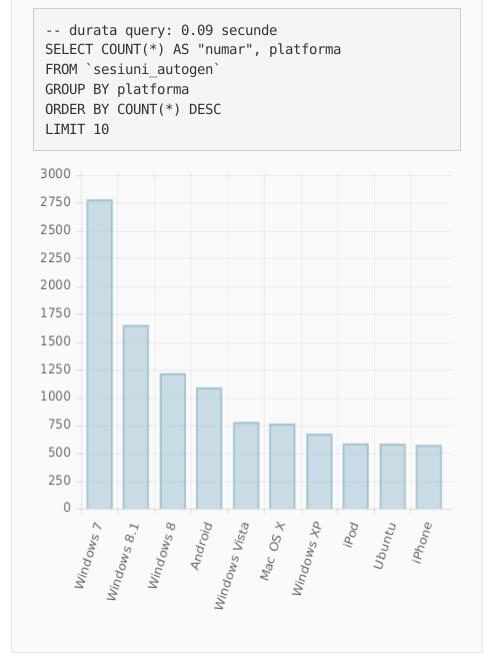
\includegraphics[width=0.50\textwidth]{img/stat.jpg}
	\vspace{-7px}
	\caption{Grafic rezultat dintr-o interogare SQL}
\end{wrapfigure}

Vizualizarea datelor joacă un rol foarte important în înțelegerea lor. \\[0.34cm]

Sistemul creează câte o vizualizare a datelor numerice rezultate dintr-o interogare SQL. Procedeul este inovativ prin faptul că se poate alipi unei infrastructuri deja existente pentru a genera grafice cu datele prezente. \\[0.34cm]

Întreaga analiză a bazelor de date poate fi găsită la adresa: \\[0.5cm]
\texttt{penultim.ddns.net/\\chatbox/statistici.php}.


\newpage
\section{Bibliografie}
\begingroup
\renewcommand{\section}[2]{}%
\begin{thebibliography}{99}

\bibitem{mysql} 
	MySQL \\
	http://www.mysql.com/about/
	
\bibitem{sgbd}
	Système de Gestion de Base de Données\\
	http://ro.wikipedia.org/wiki/Sistem\_de\_gestiune\_a\_bazelor\_de\_date

\bibitem{php}
	PHP Hypertext Processor\\
	http://php.net/manual/en/intro-whatis.php

\bibitem{pdo}
	PDO: PHP Data Objects\\
	http://php.net/manual/en/intro.pdo.php
	
\bibitem{websocket}
	Websocket Protocol\\
	https://www.websocket.org/
	
\bibitem{ratchet}
	Ratchet: a Websocket Library\\
	http://socketo.me/
	
\bibitem{javascript}
	Objects  in Javascript\\
	http://www.w3.org/community/webed/wiki/Objects\_in\_JavaScript
	
\bibitem{jquery}
	jQuery: The Write Less, Do More, JavaScript Library\\
	https://jquery.com/
	
\bibitem{dom}
	Document Object Model\\
	http://www.w3.org/DOM/

\bibitem{chartjs}
	Chart.js: Open source HTML5 Charts \\
	http://www.chartjs.org/
	
\bibitem{bootstrap}
	Bootstrap -- Designed for everyone, everywhere \\
	http://getbootstrap.com/
	
\bibitem{python}
	Python \\
	https://www.python.org/about/

\bibitem{pythonWiki}
	Python, articol Wikipedia\\
	http://ro.wikipedia.org/wiki/Python
	
\bibitem{noip}
	No-IP: a Dynamic DNS company \\
	http://www.noip.com/
	
\bibitem{debian}
	Debian GNU/Linux \\
	https://www.debian.org/intro/about

\bibitem{free}
	Software liber / Free Software \\
	https://www.fsf.org/about/what-is-free-software
	
\bibitem{apache53}
	June 2013 Web Server Survey\\
	\small{http://news.netcraft.com/archives/2013/06/06/june-2013-web-server-survey-3.html}
	
\bibitem{daemon}
	daemontools\\
	http://cr.yp.to/daemontools.html

\bibitem{passwordhash}
	PHP5 PASSWORD\_HASH\\
	http://php.net/manual/en/function.password-hash.php
	
\bibitem{uml}
	Unified Modeling Language\\
	http://www.uml.org/
	
\bibitem{bootswatch}
	Bootswatch: Free themes for Bootstrap\\
	https://bootswatch.com/
	
\bibitem{yeti}
	Bootswatch Yeti Theme: A friendly foundation\\
	https://bootswatch.com/yeti/
	
\bibitem{rwd}
	Responsive Web Design\\
	http://alistapart.com/article/responsive-web-design\\
	http://en.wikipedia.org/wiki/Responsive\_web\_design	
	

\end{thebibliography}
\endgroup
\newpage
\tableofcontents

\end{document}